\chapter*{Introduction}
\addcontentsline{toc}{chapter}{Introduction}

\section{Inertial Confinement Fusion and High-Energy-Density Physics}

Since the cessation of full-scale nuclear testing, numerical simulation has become a central tool for the study and maintenance of nuclear deterrence capabilities. In this context, understanding high-energy-density physics (HEDP) phenomena is of major importance. However, the extreme thermodynamic conditions involved in thermonuclear systems cannot be reproduced using conventional laboratory experiments. As a consequence, dedicated experimental platforms are required to investigate these physical regimes and validate numerical models.

Among these platforms, Inertial Confinement Fusion (ICF) constitutes one of the most important experimental frameworks for the study of compressible plasma dynamics, shock propagation, radiation transport, and hydrodynamic instabilities under extreme conditions. Although initially developed in the context of controlled fusion research, ICF experiments also provide access to physical regimes relevant to astrophysics and nuclear weapons physics.

In inertial confinement fusion, a small spherical capsule containing deuterium--tritium fuel is rapidly compressed using high-intensity laser beams. The outer shell of the target is heated and ablated, generating an inward-directed pressure that compresses the fuel to extremely high temperatures and densities. Under sufficiently symmetric compression conditions, thermonuclear reactions may occur before the target disassembles due to its own expansion.

\begin{figure}[h]
\centering
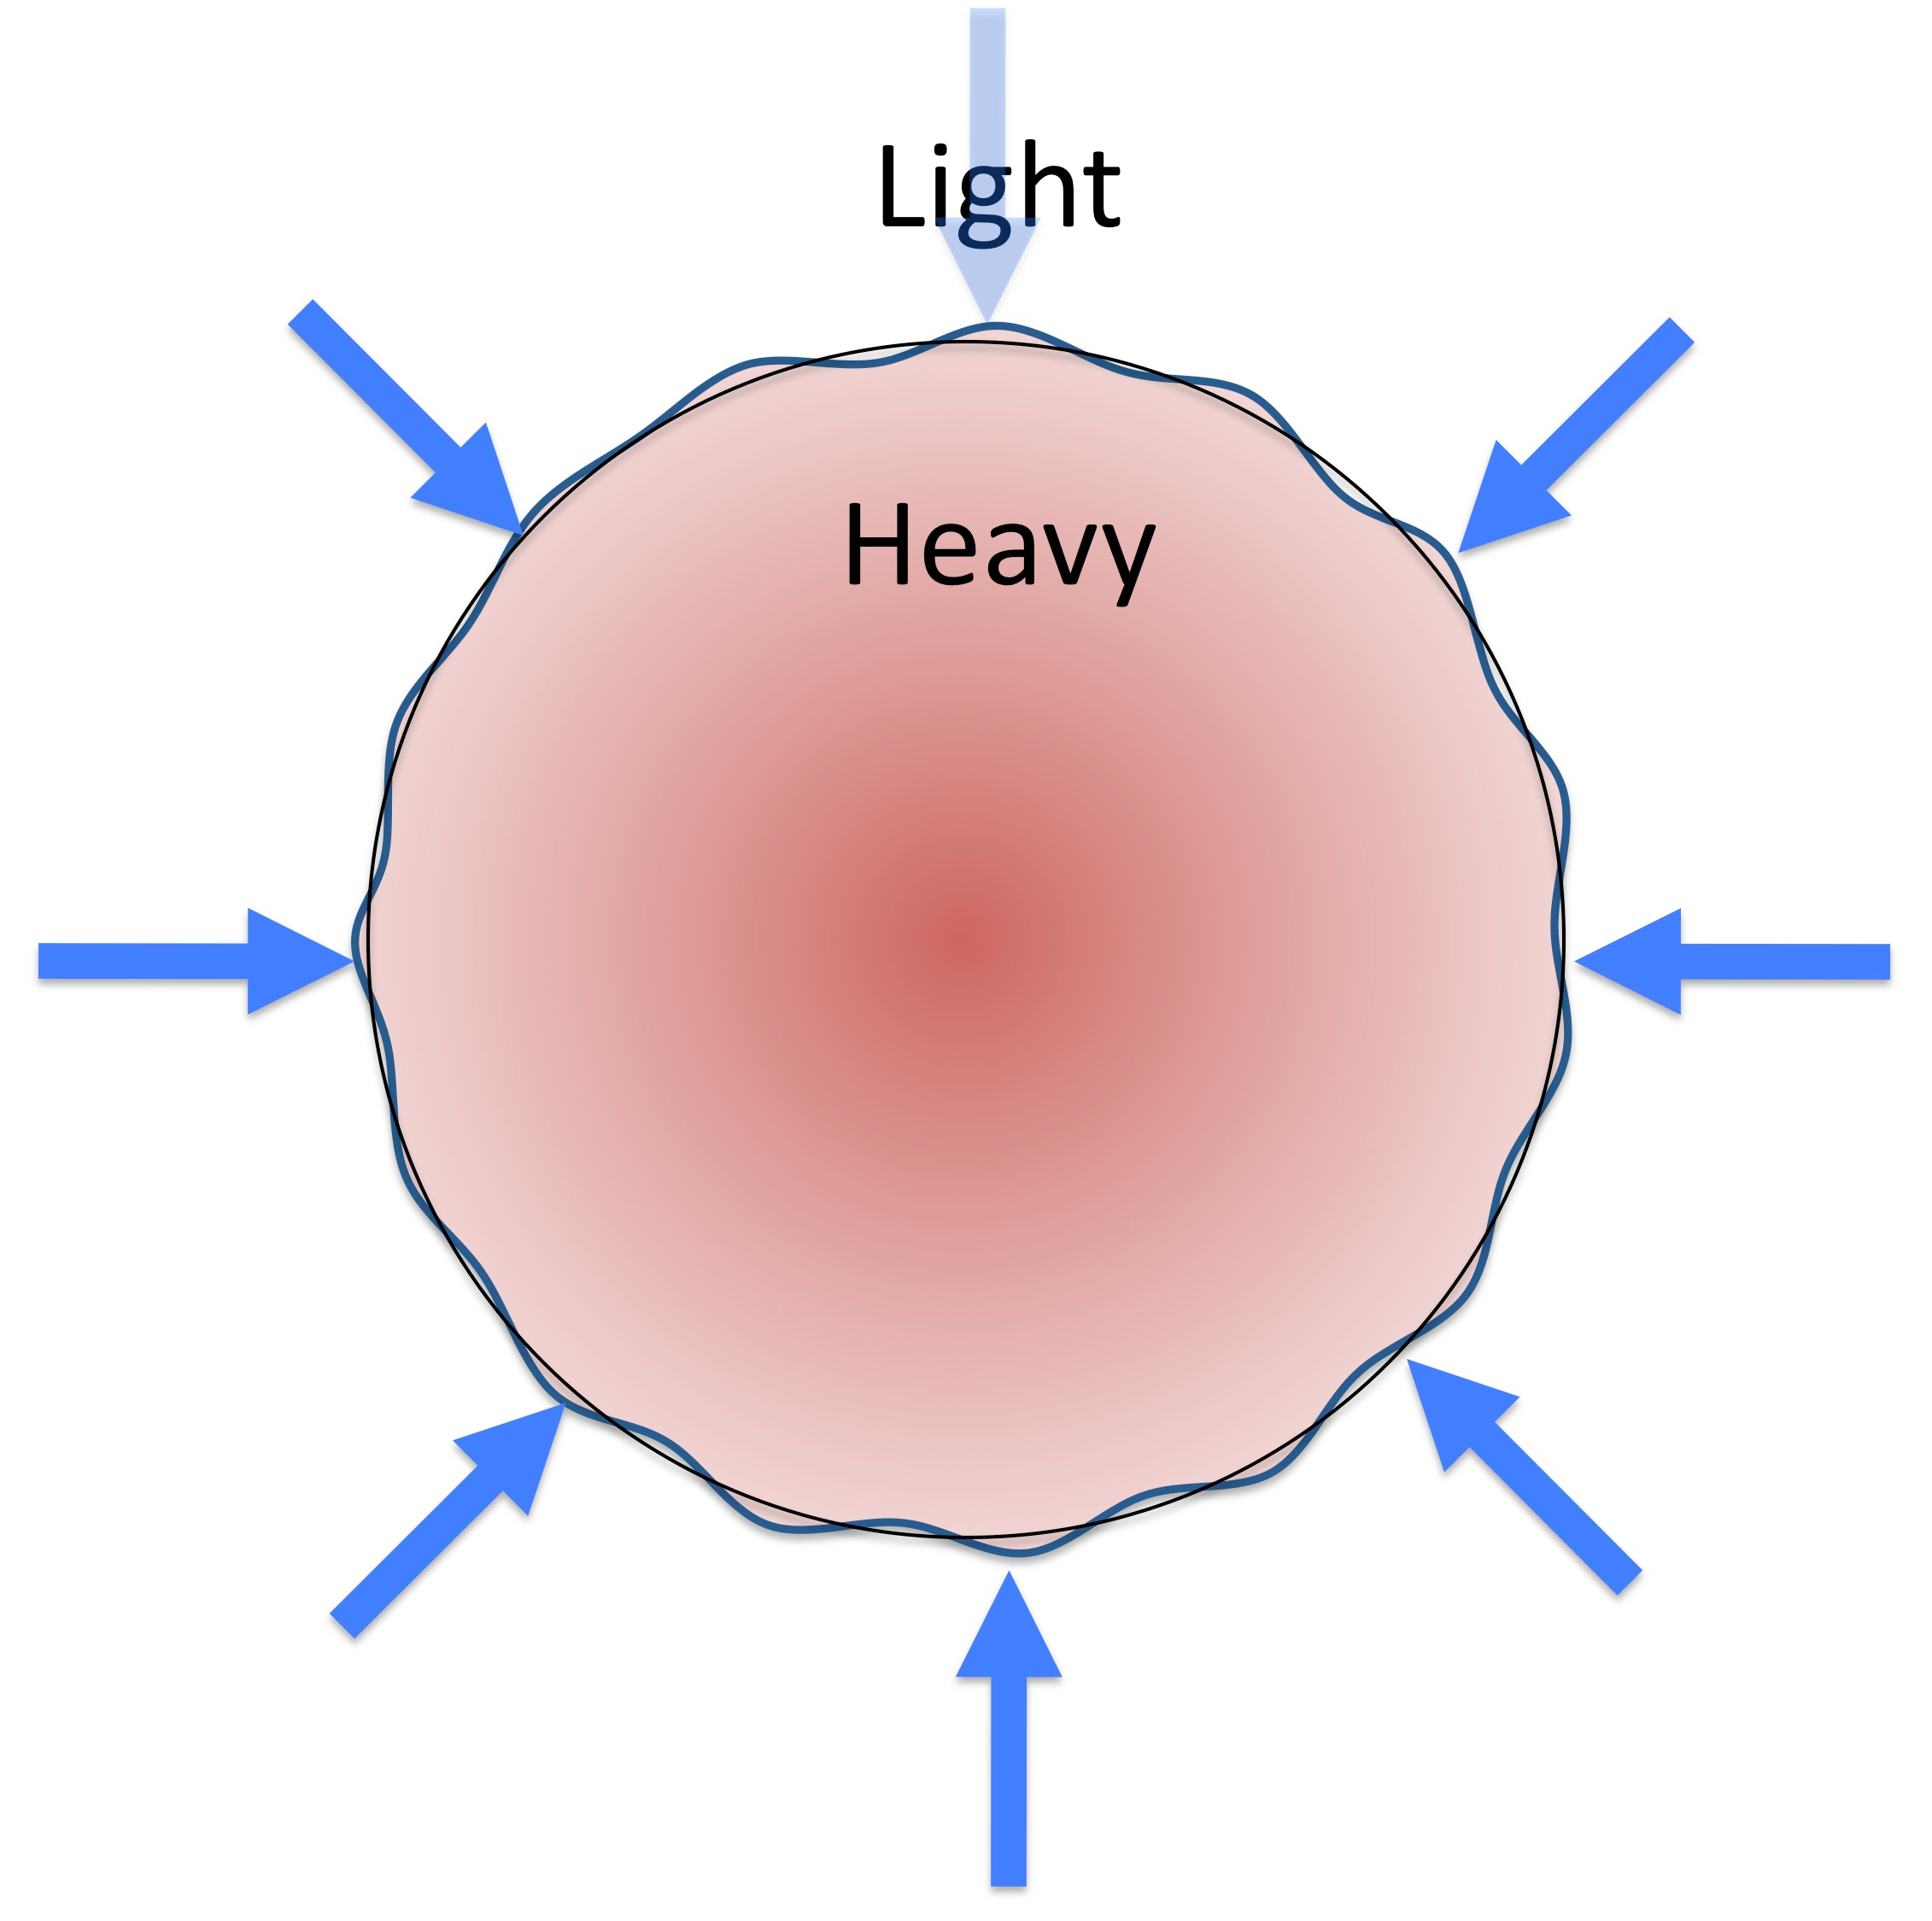
\includegraphics[width=0.40\textwidth]{figures/intro/fci.png}
\caption{Schematic representation of an inertial confinement fusion target and laser-driven implosion process.}
\label{fig:icf_principle}
\end{figure}

One of the main scientific challenges in ICF is maintaining the symmetry and stability of the implosion during compression. Small perturbations located at material interfaces may grow rapidly and strongly deteriorate the implosion quality. These effects are primarily driven by hydrodynamic instabilities, among which the Rayleigh--Taylor instability plays a significant role.

\section{Rayleigh--Taylor Instability in ICF}

The Rayleigh--Taylor instability (RTI) occurs when a denser fluid is accelerated by a lighter one. In inertial confinement fusion configurations, the hot ablated plasma accelerates the denser shell material inward during the implosion process. Under these conditions, small imperfections initially present on the capsule surface grow rapidly and progressively distort the interface.

\begin{figure}[h]
\centering

\includegraphics[width=0.85\textwidth]{figures/intro/rti_sketch.png}
\caption{Illustration of the Rayleigh--Taylor instability developing at the interface between two fluids of different densities.}
\label{fig:rti_scheme}
\end{figure}

As the instability evolves, the interface develops characteristic bubble and spike structures which eventually transition toward a turbulent mixing regime. This turbulent mixing degrades the compression efficiency, reduces the achievable temperature in the fuel core, and may ultimately prevent ignition conditions from being reached. Consequently, understanding and predicting RTI growth is a critical challenge for inertial confinement fusion and high-energy-density plasma physics.

From a mathematical perspective, RTI dynamics are governed by the compressible Navier--Stokes equations coupled with thermodynamic and transport models. Due to the highly non-linear and multi-scale nature of the phenomenon, analytical approaches remain limited to simplified configurations and early linear growth regimes. Realistic configurations therefore require large-scale numerical simulations capable of accurately resolving the instability dynamics.

\section{Direct Numerical Simulations and Dataset Generation}

To investigate the evolution of the Rayleigh--Taylor instability, Direct Numerical Simulations (DNS) are requiered due to the lack of 
closure equation in the turbulence transition phase. Therefore in this work, the dataset is generated using DNS, which explicitly resolve all relevant spatial and temporal scales of the flow without relying on turbulence models.

DNS provides highly accurate representations of instability growth and enables detailed observation of the transition from the linear regime toward fully developed turbulent mixing. Such simulations constitute valuable reference data both for physical analysis and for the validation of reduced-order or data-driven models.

However, the computational cost associated with DNS remains extremely high. Accurately resolving fine-scale turbulent structures requires very large computational grids and significant execution times on high-performance computing infrastructures. Consequently, only a very limited number of simulations can generally be produced.

\begin{figure}[h]
\centering
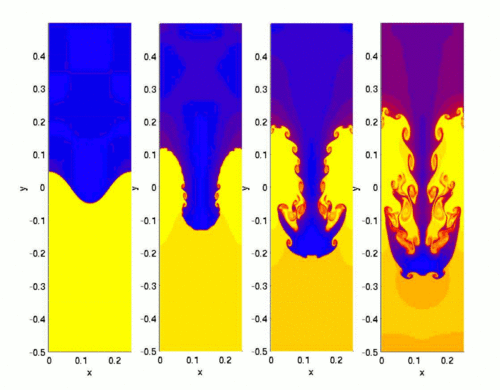
\includegraphics[width=0.85\textwidth]{figures/intro/rti.png}
\caption{Example of density fields evolution obtained from Direct Numerical Simulations of the Rayleigh--Taylor instability.}
\label{fig:dns_example}
\end{figure}

This limitation motivates the development of surrogate or meta-modeling approaches capable of approximating the statistical and dynamical behavior of DNS simulations while drastically reducing computational costs. In recent years, machine learning methods have emerged as promising tools for the construction of surrogate models in computational fluid dynamics and plasma physics applications.

\section{Machine Learning and Diffusion-Based Surrogate Modeling}

Recent advances in generative artificial intelligence, and more specifically diffusion models, have demonstrated remarkable capabilities for learning complex high-dimensional probability distributions. Initially developed for image synthesis applications, diffusion models are now increasingly investigated for scientific computing problems involving stochastic and multi-scale physical systems.

In the present work, the objective is to develop a diffusion-based surrogate model capable of approximating the probability distribution associated with two-dimensional Rayleigh--Taylor instability simulations. Due to the limited amount of DNS data available, particular attention is given to wavelet-based diffusion approaches, which exploit multi-scale representations of physical fields in order to improve data efficiency and reconstruction quality.

The proposed methodology is inspired by recent work on wavelet diffusion models and aims at evaluating whether such architectures can provide improved generalization capabilities compared to conventional diffusion approaches when trained on limited scientific datasets.

\begin{figure}[h]
\centering
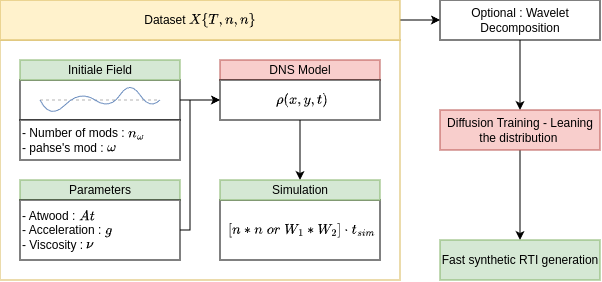
\includegraphics[width=0.85\textwidth]{figures/intro/pipeline_sktech.drawio.png}
\caption{General principle of the diffusion-based surrogate modeling approach used in this work.}
\label{fig:diffusion_pipeline}
\end{figure}

\section{Contributions}
\begin{todobox}
Ajouter ici une explication breve des contributions apportées durant le stage
\end{todobox}
